% 87-74(87쪽) — AB=8, BC=9, ∠B=45°인 삼각형 ABC 와 변 AB·BC 위를 움직이는 두 점 P, Q(삼각형 PBQ 색칠). 스캔 화질이 낮아 TikZ 로 다시 그림.
% 원문에 있는 것만: 삼각형 ABC · 선분 PQ · 색칠한 삼각형 PBQ · 8 과 9 를 가리키는 파선 호 · 45° 표시 · 두 점이 움직이는 방향 화살표 · 라벨 A, B, C, P, Q.
% BP·BQ 의 값은 원문에 없으므로 적지 않는다(2초 후의 넓이의 변화율이 그림에서 읽히지 않게).
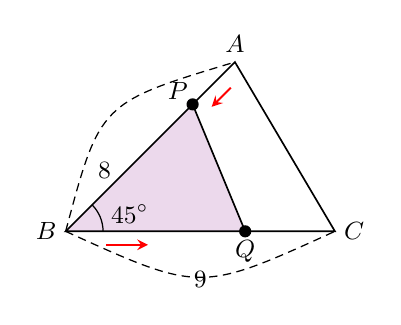
\begin{tikzpicture}[x=0.38cm, y=0.38cm, line width=0.55pt]
  \fill[violet!15] (0,0) -- (4.243,4.243) -- (6,0) -- cycle;
  \draw[line width=0.6pt] (0,0) -- (5.657,5.657) -- (9,0) -- cycle;
  \draw[line width=0.6pt] (4.243,4.243) -- (6,0);
  % 45° 표시
  \draw[line width=0.45pt] (1.25,0) arc (0:45:1.25);
  \node[anchor=west, inner sep=1pt, font=\small] at (1.40,0.58) {$45^\circ$};
  % 8 · 9 를 가리키는 파선 호
  \draw[densely dashed, line width=0.45pt] (0,0) .. controls (1.15,4.30) .. (5.657,5.657);
  \draw[densely dashed, line width=0.45pt] (0,0) .. controls (4.5,-2.05) .. (9,0);
  \node[font=\small] at (1.30,2.05) {$8$};
  \node[font=\small] at (4.50,-1.60) {$9$};
  % 두 점이 움직이는 방향(원문의 화살표)
  \draw[->, >=stealth, red, line width=0.7pt] (5.52,4.80) -- (4.88,4.16);
  \draw[->, >=stealth, red, line width=0.7pt] (1.35,-0.45) -- (2.75,-0.45);
  \fill (4.243,4.243) circle (2.2pt);
  \fill (6,0) circle (2.2pt);
  \node[anchor=south, inner sep=3pt, font=\small] at (5.657,5.657) {$\pt{A}$};
  \node[anchor=east, inner sep=3pt, font=\small] at (0,0) {$\pt{B}$};
  \node[anchor=west, inner sep=3pt, font=\small] at (9,0) {$\pt{C}$};
  \node[anchor=south east, inner sep=1.5pt, font=\small] at (4.243,4.243) {$\pt{P}$};
  \node[anchor=north, inner sep=3pt, font=\small] at (6,0) {$\pt{Q}$};
\end{tikzpicture}
